\section{Use case} \label{sec:usecase} 
På baggrund af opstillet krav i \autoref{sec:funktionellekrav} er der udarbejdet et use case diagram, der beskriver app'ens funktioner. Af use case diagrammet på \autoref{fig:usecase} ses systemet, de forskellige use cases og aktører der kan interagere med systemet. KOL-patienten er den primære aktør, som kan tilgå alle use cases. Målinger, andre KOL-patienter, sundhedspersonale og database er sekundære aktører og kan kun tilgå få use cases. 

\begin{figure} [H]
\centering
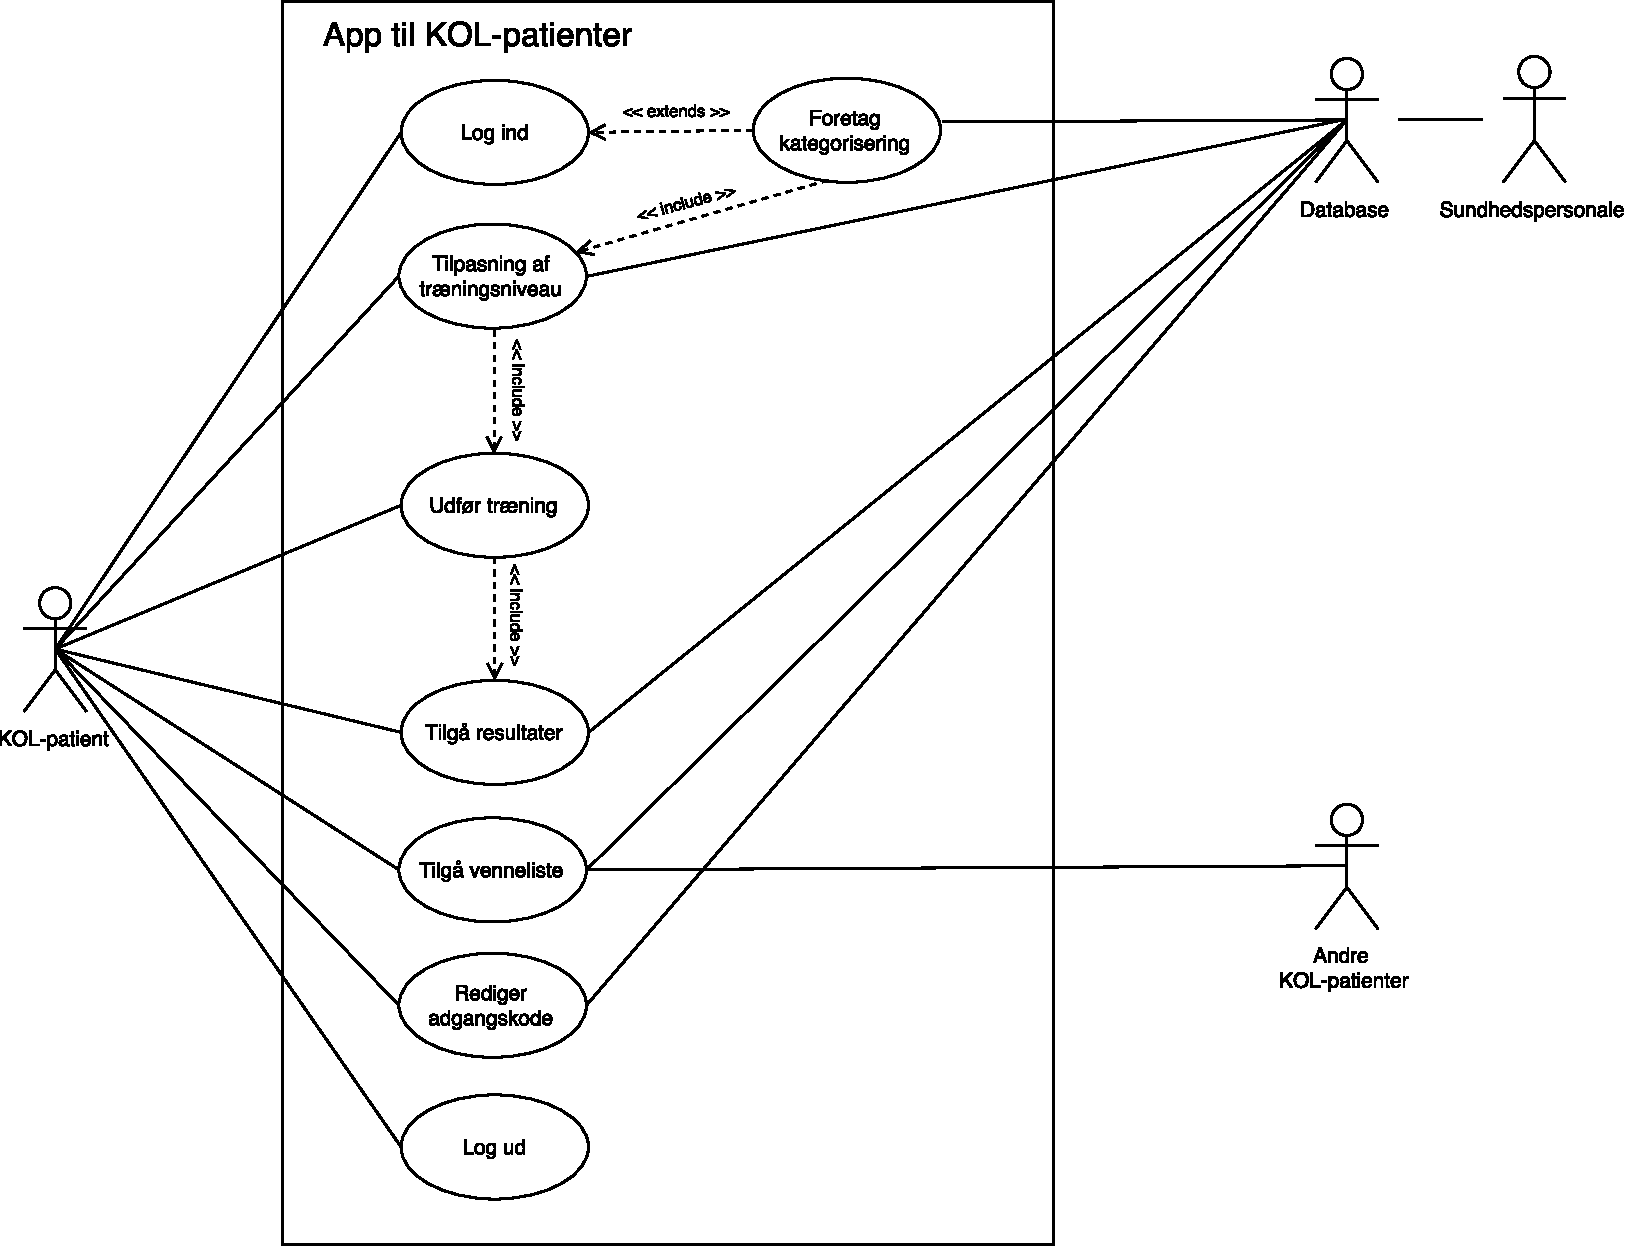
\includegraphics[width=0.9\textwidth]{figures/aktivitetsdiagram/Usecase}
\caption{Use case for app til KOL-patienter}
\label{fig:usecase}
\end{figure}

\noindent
Efter KOL-patienter er logget ind i app'en har de adgang til en hovedmenu, hvor patienter kan redigere brugeroplysninger, udføre træning, se resultater og venneliste. 


I brugeroplysninger kan patienter redigere deres adgangskode og kategorisering. Ændringer gemmes efterfølgende i databasen. 

Patienten kan udføre træningen som tilpasses individuelt alt efter niveau. Niveauet bestemmes ud fra den enkelte patients status som vurderes ud fra kategorisering, den daglige helbredstilstand og evalueringen af tidligere træninger. 
Undertræningen kan eksterne enheder tilkobles systemet så fysiologiske målinger kan opsamles. Efter fuldført træningen gemmes patientstatus, trænings resultater og målinger i resultater og databasen. Herefter startes en nedtælling som nulstilles efter 24 timer eller ved fuldført træning. Påbegyndes træningen ikke inden for 24 timer sendes en notifikation. 


KOL-patienter tilgå samtlige resultater, som visualiseres på forskellige måder. Sundhedspersonalet kan kun følge med i udviklingen af KOL-patienten. Andre KOL-patienter kan tilgå resultater via. vennelisten. I vennelisten kan KOL-patienter tilføje, slette og vælge andre KOL-patienter samt se deres belønninger..... 



